% Created by tikzDevice version 0.10.1 on 2016-06-16 17:59:36
% !TEX encoding = UTF-8 Unicode
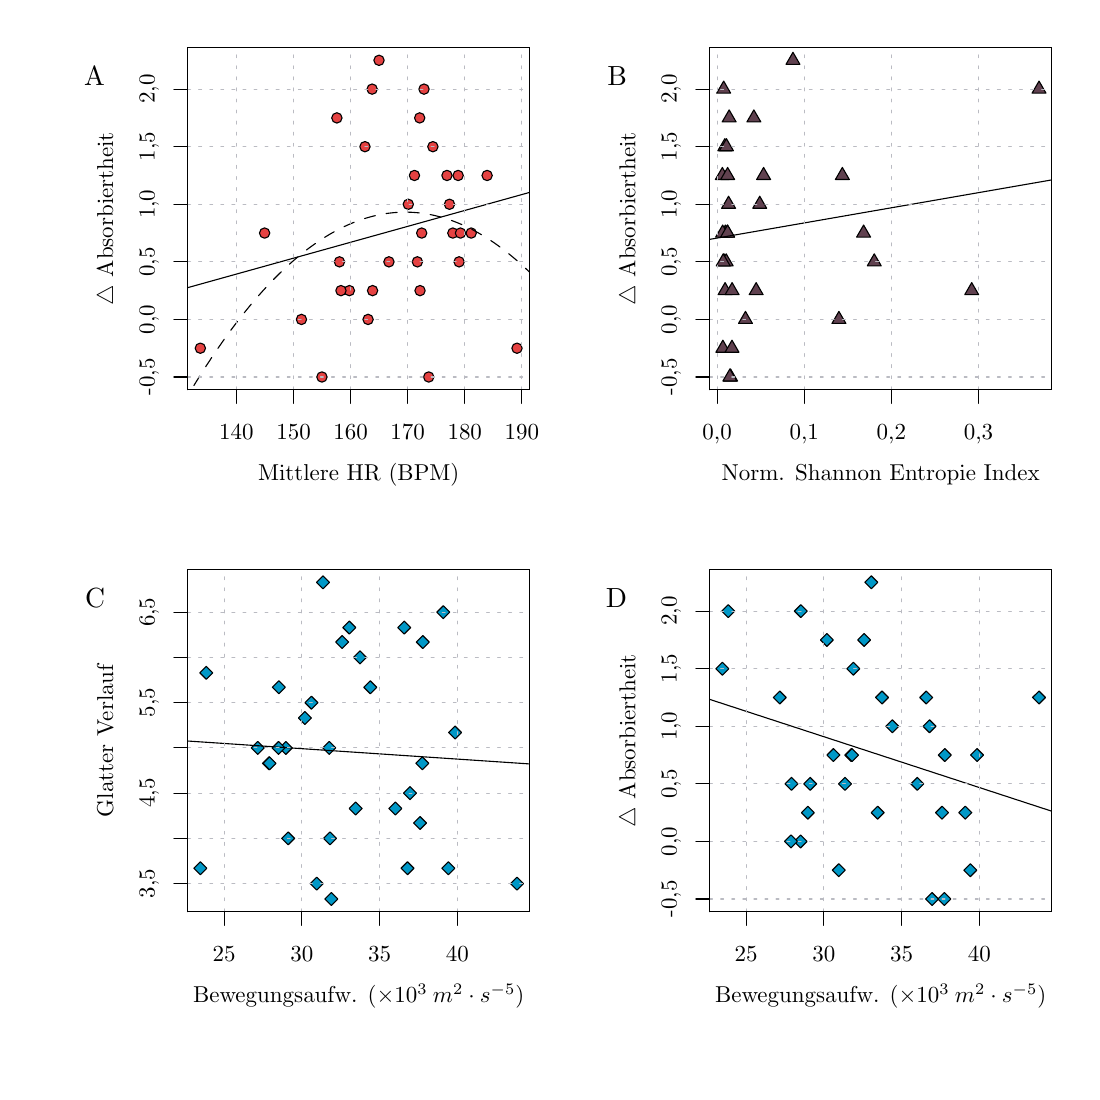
\begin{tikzpicture}[x=1pt,y=1pt]
\definecolor{fillColor}{RGB}{255,255,255}
\path[use as bounding box,fill=fillColor,fill opacity=0.00] (0,0) rectangle (377.25,377.25);
\begin{scope}
\path[clip] ( 57.82,246.44) rectangle (181.40,370.02);
\definecolor{drawColor}{RGB}{0,0,0}
\definecolor{fillColor}{RGB}{229,66,66}

\path[draw=drawColor,line width= 0.4pt,line join=round,line cap=round,fill=fillColor] (116.25,282.23) circle (  1.87);

\path[draw=drawColor,line width= 0.4pt,line join=round,line cap=round,fill=fillColor] (155.55,323.84) circle (  1.87);

\path[draw=drawColor,line width= 0.4pt,line join=round,line cap=round,fill=fillColor] (160.27,303.03) circle (  1.87);

\path[draw=drawColor,line width= 0.4pt,line join=round,line cap=round,fill=fillColor] ( 85.62,303.03) circle (  1.87);

\path[draw=drawColor,line width= 0.4pt,line join=round,line cap=round,fill=fillColor] (137.53,313.43) circle (  1.87);

\path[draw=drawColor,line width= 0.4pt,line join=round,line cap=round,fill=fillColor] (123.00,271.82) circle (  1.87);

\path[draw=drawColor,line width= 0.4pt,line join=round,line cap=round,fill=fillColor] (126.96,365.45) circle (  1.87);

\path[draw=drawColor,line width= 0.4pt,line join=round,line cap=round,fill=fillColor] (155.89,292.63) circle (  1.87);

\path[draw=drawColor,line width= 0.4pt,line join=round,line cap=round,fill=fillColor] (176.82,261.42) circle (  1.87);

\path[draw=drawColor,line width= 0.4pt,line join=round,line cap=round,fill=fillColor] (153.63,303.03) circle (  1.87);

\path[draw=drawColor,line width= 0.4pt,line join=round,line cap=round,fill=fillColor] (166.02,323.84) circle (  1.87);

\path[draw=drawColor,line width= 0.4pt,line join=round,line cap=round,fill=fillColor] (141.66,344.64) circle (  1.87);

\path[draw=drawColor,line width= 0.4pt,line join=round,line cap=round,fill=fillColor] (141.78,282.23) circle (  1.87);

\path[draw=drawColor,line width= 0.4pt,line join=round,line cap=round,fill=fillColor] (130.54,292.63) circle (  1.87);

\path[draw=drawColor,line width= 0.4pt,line join=round,line cap=round,fill=fillColor] ( 98.93,271.82) circle (  1.87);

\path[draw=drawColor,line width= 0.4pt,line join=round,line cap=round,fill=fillColor] (146.42,334.24) circle (  1.87);

\path[draw=drawColor,line width= 0.4pt,line join=round,line cap=round,fill=fillColor] (144.92,251.02) circle (  1.87);

\path[draw=drawColor,line width= 0.4pt,line join=round,line cap=round,fill=fillColor] (111.73,344.64) circle (  1.87);

\path[draw=drawColor,line width= 0.4pt,line join=round,line cap=round,fill=fillColor] (113.20,282.23) circle (  1.87);

\path[draw=drawColor,line width= 0.4pt,line join=round,line cap=round,fill=fillColor] (139.76,323.84) circle (  1.87);

\path[draw=drawColor,line width= 0.4pt,line join=round,line cap=round,fill=fillColor] (121.88,334.24) circle (  1.87);

\path[draw=drawColor,line width= 0.4pt,line join=round,line cap=round,fill=fillColor] (124.47,355.04) circle (  1.87);

\path[draw=drawColor,line width= 0.4pt,line join=round,line cap=round,fill=fillColor] (124.63,282.23) circle (  1.87);

\path[draw=drawColor,line width= 0.4pt,line join=round,line cap=round,fill=fillColor] (112.66,292.63) circle (  1.87);

\path[draw=drawColor,line width= 0.4pt,line join=round,line cap=round,fill=fillColor] (142.38,303.03) circle (  1.87);

\path[draw=drawColor,line width= 0.4pt,line join=round,line cap=round,fill=fillColor] (151.51,323.84) circle (  1.87);

\path[draw=drawColor,line width= 0.4pt,line join=round,line cap=round,fill=fillColor] (106.33,251.02) circle (  1.87);

\path[draw=drawColor,line width= 0.4pt,line join=round,line cap=round,fill=fillColor] (152.42,313.43) circle (  1.87);

\path[draw=drawColor,line width= 0.4pt,line join=round,line cap=round,fill=fillColor] (140.82,292.63) circle (  1.87);

\path[draw=drawColor,line width= 0.4pt,line join=round,line cap=round,fill=fillColor] (143.22,355.04) circle (  1.87);

\path[draw=drawColor,line width= 0.4pt,line join=round,line cap=round,fill=fillColor] ( 62.39,261.42) circle (  1.87);

\path[draw=drawColor,line width= 0.4pt,line join=round,line cap=round,fill=fillColor] (156.39,303.03) circle (  1.87);
\end{scope}
\begin{scope}
\path[clip] (  0.00,  0.00) rectangle (377.25,377.25);
\definecolor{drawColor}{RGB}{0,0,0}

\path[draw=drawColor,line width= 0.4pt,line join=round,line cap=round] ( 75.45,246.44) -- (178.56,246.44);

\path[draw=drawColor,line width= 0.4pt,line join=round,line cap=round] ( 75.45,246.44) -- ( 75.45,241.46);

\path[draw=drawColor,line width= 0.4pt,line join=round,line cap=round] ( 96.07,246.44) -- ( 96.07,241.46);

\path[draw=drawColor,line width= 0.4pt,line join=round,line cap=round] (116.69,246.44) -- (116.69,241.46);

\path[draw=drawColor,line width= 0.4pt,line join=round,line cap=round] (137.31,246.44) -- (137.31,241.46);

\path[draw=drawColor,line width= 0.4pt,line join=round,line cap=round] (157.94,246.44) -- (157.94,241.46);

\path[draw=drawColor,line width= 0.4pt,line join=round,line cap=round] (178.56,246.44) -- (178.56,241.46);

\node[text=drawColor,anchor=base,inner sep=0pt, outer sep=0pt, scale=  0.83] at ( 75.45,228.51) {140};

\node[text=drawColor,anchor=base,inner sep=0pt, outer sep=0pt, scale=  0.83] at ( 96.07,228.51) {150};

\node[text=drawColor,anchor=base,inner sep=0pt, outer sep=0pt, scale=  0.83] at (116.69,228.51) {160};

\node[text=drawColor,anchor=base,inner sep=0pt, outer sep=0pt, scale=  0.83] at (137.31,228.51) {170};

\node[text=drawColor,anchor=base,inner sep=0pt, outer sep=0pt, scale=  0.83] at (157.94,228.51) {180};

\node[text=drawColor,anchor=base,inner sep=0pt, outer sep=0pt, scale=  0.83] at (178.56,228.51) {190};

\path[draw=drawColor,line width= 0.4pt,line join=round,line cap=round] ( 57.82,251.02) -- ( 57.82,355.04);

\path[draw=drawColor,line width= 0.4pt,line join=round,line cap=round] ( 57.82,251.02) -- ( 52.84,251.02);

\path[draw=drawColor,line width= 0.4pt,line join=round,line cap=round] ( 57.82,271.82) -- ( 52.84,271.82);

\path[draw=drawColor,line width= 0.4pt,line join=round,line cap=round] ( 57.82,292.63) -- ( 52.84,292.63);

\path[draw=drawColor,line width= 0.4pt,line join=round,line cap=round] ( 57.82,313.43) -- ( 52.84,313.43);

\path[draw=drawColor,line width= 0.4pt,line join=round,line cap=round] ( 57.82,334.24) -- ( 52.84,334.24);

\path[draw=drawColor,line width= 0.4pt,line join=round,line cap=round] ( 57.82,355.04) -- ( 52.84,355.04);

\node[text=drawColor,rotate= 90.00,anchor=base,inner sep=0pt, outer sep=0pt, scale=  0.83] at ( 45.86,251.02) {-0,5};

\node[text=drawColor,rotate= 90.00,anchor=base,inner sep=0pt, outer sep=0pt, scale=  0.83] at ( 45.86,271.82) {0,0};

\node[text=drawColor,rotate= 90.00,anchor=base,inner sep=0pt, outer sep=0pt, scale=  0.83] at ( 45.86,292.63) {0,5};

\node[text=drawColor,rotate= 90.00,anchor=base,inner sep=0pt, outer sep=0pt, scale=  0.83] at ( 45.86,313.43) {1,0};

\node[text=drawColor,rotate= 90.00,anchor=base,inner sep=0pt, outer sep=0pt, scale=  0.83] at ( 45.86,334.24) {1,5};

\node[text=drawColor,rotate= 90.00,anchor=base,inner sep=0pt, outer sep=0pt, scale=  0.83] at ( 45.86,355.04) {2,0};

\path[draw=drawColor,line width= 0.4pt,line join=round,line cap=round] ( 57.82,246.44) --
	(181.40,246.44) --
	(181.40,370.02) --
	( 57.82,370.02) --
	( 57.82,246.44);
\end{scope}
\begin{scope}
\path[clip] (  0.00,188.62) rectangle (188.62,377.25);
\definecolor{drawColor}{RGB}{0,0,0}

\node[text=drawColor,anchor=base,inner sep=0pt, outer sep=0pt, scale=  0.83] at (119.61,213.57) {Mittlere HR (BPM)};

\node[text=drawColor,rotate= 90.00,anchor=base,inner sep=0pt, outer sep=0pt, scale=  0.83] at ( 30.92,308.23) {$\bigtriangleup$ Absorbiertheit};
\end{scope}
\begin{scope}
\path[clip] ( 57.82,246.44) rectangle (181.40,370.02);
\definecolor{drawColor}{RGB}{0,0,0}

\path[draw=drawColor,line width= 0.4pt,line join=round,line cap=round] ( 57.82,283.30) -- (181.40,317.73);

\path[draw=drawColor,line width= 0.4pt,dash pattern=on 4pt off 4pt ,line join=round,line cap=round] ( 34.20,198.31) --
	( 35.23,200.57) --
	( 36.26,202.80) --
	( 37.30,205.01) --
	( 38.33,207.19) --
	( 39.36,209.35) --
	( 40.39,211.49) --
	( 41.42,213.61) --
	( 42.45,215.70) --
	( 43.48,217.77) --
	( 44.51,219.82) --
	( 45.54,221.85) --
	( 46.58,223.85) --
	( 47.61,225.83) --
	( 48.64,227.78) --
	( 49.67,229.72) --
	( 50.70,231.63) --
	( 51.73,233.52) --
	( 52.76,235.38) --
	( 53.79,237.22) --
	( 54.82,239.04) --
	( 55.86,240.84) --
	( 56.89,242.61) --
	( 57.92,244.36) --
	( 58.95,246.09) --
	( 59.98,247.80) --
	( 61.01,249.48) --
	( 62.04,251.14) --
	( 63.07,252.77) --
	( 64.10,254.39) --
	( 65.14,255.98) --
	( 66.17,257.55) --
	( 67.20,259.09) --
	( 68.23,260.61) --
	( 69.26,262.11) --
	( 70.29,263.59) --
	( 71.32,265.05) --
	( 72.35,266.48) --
	( 73.38,267.88) --
	( 74.42,269.27) --
	( 75.45,270.63) --
	( 76.48,271.97) --
	( 77.51,273.29) --
	( 78.54,274.58) --
	( 79.57,275.85) --
	( 80.60,277.10) --
	( 81.63,278.33) --
	( 82.66,279.53) --
	( 83.70,280.71) --
	( 84.73,281.87) --
	( 85.76,283.00) --
	( 86.79,284.11) --
	( 87.82,285.20) --
	( 88.85,286.27) --
	( 89.88,287.31) --
	( 90.91,288.33) --
	( 91.94,289.33) --
	( 92.98,290.30) --
	( 94.01,291.25) --
	( 95.04,292.18) --
	( 96.07,293.08) --
	( 97.10,293.97) --
	( 98.13,294.83) --
	( 99.16,295.66) --
	(100.19,296.48) --
	(101.22,297.27) --
	(102.26,298.04) --
	(103.29,298.78) --
	(104.32,299.51) --
	(105.35,300.21) --
	(106.38,300.88) --
	(107.41,301.54) --
	(108.44,302.17) --
	(109.47,302.78) --
	(110.50,303.36) --
	(111.54,303.93) --
	(112.57,304.47) --
	(113.60,304.99) --
	(114.63,305.48) --
	(115.66,305.95) --
	(116.69,306.40) --
	(117.72,306.83) --
	(118.75,307.23) --
	(119.78,307.61) --
	(120.82,307.97) --
	(121.85,308.30) --
	(122.88,308.61) --
	(123.91,308.90) --
	(124.94,309.17) --
	(125.97,309.41) --
	(127.00,309.63) --
	(128.03,309.83) --
	(129.06,310.00) --
	(130.10,310.16) --
	(131.13,310.28) --
	(132.16,310.39) --
	(133.19,310.47) --
	(134.22,310.53) --
	(135.25,310.57) --
	(136.28,310.59) --
	(137.31,310.58) --
	(138.34,310.55) --
	(139.38,310.49) --
	(140.41,310.42) --
	(141.44,310.32) --
	(142.47,310.19) --
	(143.50,310.05) --
	(144.53,309.88) --
	(145.56,309.69) --
	(146.59,309.48) --
	(147.62,309.24) --
	(148.66,308.98) --
	(149.69,308.70) --
	(150.72,308.39) --
	(151.75,308.07) --
	(152.78,307.72) --
	(153.81,307.34) --
	(154.84,306.94) --
	(155.87,306.53) --
	(156.90,306.08) --
	(157.94,305.62) --
	(158.97,305.13) --
	(160.00,304.62) --
	(161.03,304.09) --
	(162.06,303.53) --
	(163.09,302.95) --
	(164.12,302.35) --
	(165.15,301.72) --
	(166.18,301.08) --
	(167.21,300.41) --
	(168.25,299.71) --
	(169.28,299.00) --
	(170.31,298.26) --
	(171.34,297.49) --
	(172.37,296.71) --
	(173.40,295.90) --
	(174.43,295.07) --
	(175.46,294.22) --
	(176.49,293.34) --
	(177.53,292.44) --
	(178.56,291.52) --
	(179.59,290.58) --
	(180.62,289.61) --
	(181.65,288.62) --
	(182.68,287.61) --
	(183.71,286.57) --
	(184.74,285.51) --
	(185.77,284.43) --
	(186.81,283.32) --
	(187.84,282.20) --
	(188.87,281.05) --
	(189.90,279.87) --
	(190.93,278.68) --
	(191.96,277.46) --
	(192.99,276.22) --
	(194.02,274.95) --
	(195.05,273.66) --
	(196.09,272.35) --
	(197.12,271.02) --
	(198.15,269.67) --
	(199.18,268.29);
\definecolor{drawColor}{RGB}{186,187,194}

\path[draw=drawColor,line width= 0.4pt,dash pattern=on 1pt off 3pt ,line join=round,line cap=round] ( 75.45,246.44) -- ( 75.45,370.02);

\path[draw=drawColor,line width= 0.4pt,dash pattern=on 1pt off 3pt ,line join=round,line cap=round] ( 96.07,246.44) -- ( 96.07,370.02);

\path[draw=drawColor,line width= 0.4pt,dash pattern=on 1pt off 3pt ,line join=round,line cap=round] (116.69,246.44) -- (116.69,370.02);

\path[draw=drawColor,line width= 0.4pt,dash pattern=on 1pt off 3pt ,line join=round,line cap=round] (137.31,246.44) -- (137.31,370.02);

\path[draw=drawColor,line width= 0.4pt,dash pattern=on 1pt off 3pt ,line join=round,line cap=round] (157.94,246.44) -- (157.94,370.02);

\path[draw=drawColor,line width= 0.4pt,dash pattern=on 1pt off 3pt ,line join=round,line cap=round] (178.56,246.44) -- (178.56,370.02);

\path[draw=drawColor,line width= 0.4pt,dash pattern=on 1pt off 3pt ,line join=round,line cap=round] ( 57.82,251.02) -- (181.40,251.02);

\path[draw=drawColor,line width= 0.4pt,dash pattern=on 1pt off 3pt ,line join=round,line cap=round] ( 57.82,271.82) -- (181.40,271.82);

\path[draw=drawColor,line width= 0.4pt,dash pattern=on 1pt off 3pt ,line join=round,line cap=round] ( 57.82,292.63) -- (181.40,292.63);

\path[draw=drawColor,line width= 0.4pt,dash pattern=on 1pt off 3pt ,line join=round,line cap=round] ( 57.82,313.43) -- (181.40,313.43);

\path[draw=drawColor,line width= 0.4pt,dash pattern=on 1pt off 3pt ,line join=round,line cap=round] ( 57.82,334.24) -- (181.40,334.24);

\path[draw=drawColor,line width= 0.4pt,dash pattern=on 1pt off 3pt ,line join=round,line cap=round] ( 57.82,355.04) -- (181.40,355.04);
\end{scope}
\begin{scope}
\path[clip] (  0.00,  0.00) rectangle (377.25,377.25);
\definecolor{drawColor}{RGB}{0,0,0}

\path[draw=drawColor,line width= 0.4pt,line join=round,line cap=round] ( 57.82,246.44) --
	(181.40,246.44) --
	(181.40,370.02) --
	( 57.82,370.02) --
	( 57.82,246.44);

\node[text=drawColor,anchor=base east,inner sep=0pt, outer sep=0pt, scale=  1.00] at ( 27.94,356.44) {A};
\end{scope}
\begin{scope}
\path[clip] (246.44,246.44) rectangle (370.02,370.02);
\definecolor{drawColor}{RGB}{0,0,0}
\definecolor{fillColor}{RGB}{96,65,79}

\path[draw=drawColor,line width= 0.4pt,line join=round,line cap=round,fill=fillColor] (252.01,285.13) --
	(254.52,280.77) --
	(249.49,280.77) --
	cycle;

\path[draw=drawColor,line width= 0.4pt,line join=round,line cap=round,fill=fillColor] (294.38,326.74) --
	(296.90,322.38) --
	(291.87,322.38) --
	cycle;

\path[draw=drawColor,line width= 0.4pt,line join=round,line cap=round,fill=fillColor] (252.10,305.93) --
	(254.62,301.58) --
	(249.59,301.58) --
	cycle;

\path[draw=drawColor,line width= 0.4pt,line join=round,line cap=round,fill=fillColor] (252.84,305.93) --
	(255.36,301.58) --
	(250.33,301.58) --
	cycle;

\path[draw=drawColor,line width= 0.4pt,line join=round,line cap=round,fill=fillColor] (264.53,316.34) --
	(267.04,311.98) --
	(262.01,311.98) --
	cycle;

\path[draw=drawColor,line width= 0.4pt,line join=round,line cap=round,fill=fillColor] (293.14,274.73) --
	(295.66,270.37) --
	(290.63,270.37) --
	cycle;

\path[draw=drawColor,line width= 0.4pt,line join=round,line cap=round,fill=fillColor] (276.54,368.35) --
	(279.05,363.99) --
	(274.02,363.99) --
	cycle;

\path[draw=drawColor,line width= 0.4pt,line join=round,line cap=round,fill=fillColor] (251.64,295.53) --
	(254.15,291.18) --
	(249.12,291.18) --
	cycle;

\path[draw=drawColor,line width= 0.4pt,line join=round,line cap=round,fill=fillColor] (251.21,264.32) --
	(253.72,259.97) --
	(248.69,259.97) --
	cycle;

\path[draw=drawColor,line width= 0.4pt,line join=round,line cap=round,fill=fillColor] (302.06,305.93) --
	(304.57,301.58) --
	(299.54,301.58) --
	cycle;

\path[draw=drawColor,line width= 0.4pt,line join=round,line cap=round,fill=fillColor] (265.92,326.74) --
	(268.44,322.38) --
	(263.41,322.38) --
	cycle;

\path[draw=drawColor,line width= 0.4pt,line join=round,line cap=round,fill=fillColor] (262.41,347.54) --
	(264.92,343.19) --
	(259.89,343.19) --
	cycle;

\path[draw=drawColor,line width= 0.4pt,line join=round,line cap=round,fill=fillColor] (263.23,285.13) --
	(265.75,280.77) --
	(260.72,280.77) --
	cycle;

\path[draw=drawColor,line width= 0.4pt,line join=round,line cap=round,fill=fillColor] (252.40,295.53) --
	(254.92,291.18) --
	(249.89,291.18) --
	cycle;

\path[draw=drawColor,line width= 0.4pt,line join=round,line cap=round,fill=fillColor] (259.37,274.73) --
	(261.89,270.37) --
	(256.86,270.37) --
	cycle;

\path[draw=drawColor,line width= 0.4pt,line join=round,line cap=round,fill=fillColor] (251.91,337.14) --
	(254.42,332.79) --
	(249.39,332.79) --
	cycle;

\path[draw=drawColor,line width= 0.4pt,line join=round,line cap=round,fill=fillColor] (253.99,253.92) --
	(256.50,249.57) --
	(251.47,249.57) --
	cycle;

\path[draw=drawColor,line width= 0.4pt,line join=round,line cap=round,fill=fillColor] (253.48,347.54) --
	(255.99,343.19) --
	(250.96,343.19) --
	cycle;

\path[draw=drawColor,line width= 0.4pt,line join=round,line cap=round,fill=fillColor] (341.12,285.13) --
	(343.64,280.77) --
	(338.61,280.77) --
	cycle;

\path[draw=drawColor,line width= 0.4pt,line join=round,line cap=round,fill=fillColor] (251.02,326.74) --
	(253.53,322.38) --
	(248.50,322.38) --
	cycle;

\path[draw=drawColor,line width= 0.4pt,line join=round,line cap=round,fill=fillColor] (252.50,337.14) --
	(255.01,332.79) --
	(249.98,332.79) --
	cycle;

\path[draw=drawColor,line width= 0.4pt,line join=round,line cap=round,fill=fillColor] (365.45,357.95) --
	(367.96,353.59) --
	(362.93,353.59) --
	cycle;

\path[draw=drawColor,line width= 0.4pt,line join=round,line cap=round,fill=fillColor] (254.54,285.13) --
	(257.05,280.77) --
	(252.02,280.77) --
	cycle;

\path[draw=drawColor,line width= 0.4pt,line join=round,line cap=round,fill=fillColor] (305.91,295.53) --
	(308.43,291.18) --
	(303.40,291.18) --
	cycle;

\path[draw=drawColor,line width= 0.4pt,line join=round,line cap=round,fill=fillColor] (251.13,305.93) --
	(253.64,301.58) --
	(248.61,301.58) --
	cycle;

\path[draw=drawColor,line width= 0.4pt,line join=round,line cap=round,fill=fillColor] (252.93,326.74) --
	(255.45,322.38) --
	(250.42,322.38) --
	cycle;

\path[draw=drawColor,line width= 0.4pt,line join=round,line cap=round,fill=fillColor] (253.74,253.92) --
	(256.26,249.57) --
	(251.22,249.57) --
	cycle;

\path[draw=drawColor,line width= 0.4pt,line join=round,line cap=round,fill=fillColor] (253.27,316.34) --
	(255.78,311.98) --
	(250.75,311.98) --
	cycle;

\path[draw=drawColor,line width= 0.4pt,line join=round,line cap=round,fill=fillColor] (251.33,295.53) --
	(253.84,291.18) --
	(248.81,291.18) --
	cycle;

\path[draw=drawColor,line width= 0.4pt,line join=round,line cap=round,fill=fillColor] (251.50,357.95) --
	(254.01,353.59) --
	(248.98,353.59) --
	cycle;

\path[draw=drawColor,line width= 0.4pt,line join=round,line cap=round,fill=fillColor] (254.50,264.32) --
	(257.02,259.97) --
	(251.99,259.97) --
	cycle;

\path[draw=drawColor,line width= 0.4pt,line join=round,line cap=round,fill=fillColor] (252.91,305.93) --
	(255.43,301.58) --
	(250.40,301.58) --
	cycle;
\end{scope}
\begin{scope}
\path[clip] (  0.00,  0.00) rectangle (377.25,377.25);
\definecolor{drawColor}{RGB}{0,0,0}

\path[draw=drawColor,line width= 0.4pt,line join=round,line cap=round] (249.12,246.44) -- (343.60,246.44);

\path[draw=drawColor,line width= 0.4pt,line join=round,line cap=round] (249.12,246.44) -- (249.12,241.46);

\path[draw=drawColor,line width= 0.4pt,line join=round,line cap=round] (280.61,246.44) -- (280.61,241.46);

\path[draw=drawColor,line width= 0.4pt,line join=round,line cap=round] (312.11,246.44) -- (312.11,241.46);

\path[draw=drawColor,line width= 0.4pt,line join=round,line cap=round] (343.60,246.44) -- (343.60,241.46);

\node[text=drawColor,anchor=base,inner sep=0pt, outer sep=0pt, scale=  0.83] at (249.12,228.51) {0,0};

\node[text=drawColor,anchor=base,inner sep=0pt, outer sep=0pt, scale=  0.83] at (280.61,228.51) {0,1};

\node[text=drawColor,anchor=base,inner sep=0pt, outer sep=0pt, scale=  0.83] at (312.11,228.51) {0,2};

\node[text=drawColor,anchor=base,inner sep=0pt, outer sep=0pt, scale=  0.83] at (343.60,228.51) {0,3};

\path[draw=drawColor,line width= 0.4pt,line join=round,line cap=round] (246.44,251.02) -- (246.44,355.04);

\path[draw=drawColor,line width= 0.4pt,line join=round,line cap=round] (246.44,251.02) -- (241.46,251.02);

\path[draw=drawColor,line width= 0.4pt,line join=round,line cap=round] (246.44,271.82) -- (241.46,271.82);

\path[draw=drawColor,line width= 0.4pt,line join=round,line cap=round] (246.44,292.63) -- (241.46,292.63);

\path[draw=drawColor,line width= 0.4pt,line join=round,line cap=round] (246.44,313.43) -- (241.46,313.43);

\path[draw=drawColor,line width= 0.4pt,line join=round,line cap=round] (246.44,334.24) -- (241.46,334.24);

\path[draw=drawColor,line width= 0.4pt,line join=round,line cap=round] (246.44,355.04) -- (241.46,355.04);

\node[text=drawColor,rotate= 90.00,anchor=base,inner sep=0pt, outer sep=0pt, scale=  0.83] at (234.49,251.02) {-0,5};

\node[text=drawColor,rotate= 90.00,anchor=base,inner sep=0pt, outer sep=0pt, scale=  0.83] at (234.49,271.82) {0,0};

\node[text=drawColor,rotate= 90.00,anchor=base,inner sep=0pt, outer sep=0pt, scale=  0.83] at (234.49,292.63) {0,5};

\node[text=drawColor,rotate= 90.00,anchor=base,inner sep=0pt, outer sep=0pt, scale=  0.83] at (234.49,313.43) {1,0};

\node[text=drawColor,rotate= 90.00,anchor=base,inner sep=0pt, outer sep=0pt, scale=  0.83] at (234.49,334.24) {1,5};

\node[text=drawColor,rotate= 90.00,anchor=base,inner sep=0pt, outer sep=0pt, scale=  0.83] at (234.49,355.04) {2,0};

\path[draw=drawColor,line width= 0.4pt,line join=round,line cap=round] (246.44,246.44) --
	(370.02,246.44) --
	(370.02,370.02) --
	(246.44,370.02) --
	(246.44,246.44);
\end{scope}
\begin{scope}
\path[clip] (188.62,188.62) rectangle (377.25,377.25);
\definecolor{drawColor}{RGB}{0,0,0}

\node[text=drawColor,anchor=base,inner sep=0pt, outer sep=0pt, scale=  0.83] at (308.23,213.57) {Norm. Shannon Entropie Index};

\node[text=drawColor,rotate= 90.00,anchor=base,inner sep=0pt, outer sep=0pt, scale=  0.83] at (219.55,308.23) {$\bigtriangleup$ Absorbiertheit};
\end{scope}
\begin{scope}
\path[clip] (246.44,246.44) rectangle (370.02,370.02);
\definecolor{drawColor}{RGB}{0,0,0}

\path[draw=drawColor,line width= 0.4pt,line join=round,line cap=round] (246.44,300.75) -- (370.02,322.23);
\definecolor{drawColor}{RGB}{186,187,194}

\path[draw=drawColor,line width= 0.4pt,dash pattern=on 1pt off 3pt ,line join=round,line cap=round] (249.12,246.44) -- (249.12,370.02);

\path[draw=drawColor,line width= 0.4pt,dash pattern=on 1pt off 3pt ,line join=round,line cap=round] (280.61,246.44) -- (280.61,370.02);

\path[draw=drawColor,line width= 0.4pt,dash pattern=on 1pt off 3pt ,line join=round,line cap=round] (312.11,246.44) -- (312.11,370.02);

\path[draw=drawColor,line width= 0.4pt,dash pattern=on 1pt off 3pt ,line join=round,line cap=round] (343.60,246.44) -- (343.60,370.02);

\path[draw=drawColor,line width= 0.4pt,dash pattern=on 1pt off 3pt ,line join=round,line cap=round] (246.44,251.02) -- (370.02,251.02);

\path[draw=drawColor,line width= 0.4pt,dash pattern=on 1pt off 3pt ,line join=round,line cap=round] (246.44,271.82) -- (370.02,271.82);

\path[draw=drawColor,line width= 0.4pt,dash pattern=on 1pt off 3pt ,line join=round,line cap=round] (246.44,292.63) -- (370.02,292.63);

\path[draw=drawColor,line width= 0.4pt,dash pattern=on 1pt off 3pt ,line join=round,line cap=round] (246.44,313.43) -- (370.02,313.43);

\path[draw=drawColor,line width= 0.4pt,dash pattern=on 1pt off 3pt ,line join=round,line cap=round] (246.44,334.24) -- (370.02,334.24);

\path[draw=drawColor,line width= 0.4pt,dash pattern=on 1pt off 3pt ,line join=round,line cap=round] (246.44,355.04) -- (370.02,355.04);
\end{scope}
\begin{scope}
\path[clip] (  0.00,  0.00) rectangle (377.25,377.25);
\definecolor{drawColor}{RGB}{0,0,0}

\path[draw=drawColor,line width= 0.4pt,line join=round,line cap=round] (246.44,246.44) --
	(370.02,246.44) --
	(370.02,370.02) --
	(246.44,370.02) --
	(246.44,246.44);

\node[text=drawColor,anchor=base east,inner sep=0pt, outer sep=0pt, scale=  1.00] at (216.56,356.44) {B};
\end{scope}
\begin{scope}
\path[clip] ( 57.82, 57.82) rectangle (181.40,181.40);
\definecolor{drawColor}{RGB}{0,0,0}
\definecolor{fillColor}{RGB}{0,152,199}

\path[draw=drawColor,line width= 0.4pt,line join=round,line cap=round,fill=fillColor] ( 93.29,114.65) --
	( 95.64,116.99) --
	( 93.29,119.33) --
	( 90.95,116.99) --
	cycle;

\path[draw=drawColor,line width= 0.4pt,line join=round,line cap=round,fill=fillColor] (136.05,158.13) --
	(138.39,160.47) --
	(136.05,162.81) --
	(133.71,160.47) --
	cycle;

\path[draw=drawColor,line width= 0.4pt,line join=round,line cap=round,fill=fillColor] (102.53,131.00) --
	(104.87,133.34) --
	(102.53,135.68) --
	(100.19,133.34) --
	cycle;

\path[draw=drawColor,line width= 0.4pt,line join=round,line cap=round,fill=fillColor] (142.78,152.90) --
	(145.12,155.24) --
	(142.78,157.58) --
	(140.44,155.24) --
	cycle;

\path[draw=drawColor,line width= 0.4pt,line join=round,line cap=round,fill=fillColor] (123.80,136.56) --
	(126.14,138.90) --
	(123.80,141.24) --
	(121.46,138.90) --
	cycle;

\path[draw=drawColor,line width= 0.4pt,line join=round,line cap=round,fill=fillColor] ( 90.66,114.65) --
	( 93.00,116.99) --
	( 90.66,119.33) --
	( 88.32,116.99) --
	cycle;

\path[draw=drawColor,line width= 0.4pt,line join=round,line cap=round,fill=fillColor] (116.23,158.13) --
	(118.57,160.47) --
	(116.23,162.81) --
	(113.89,160.47) --
	cycle;

\path[draw=drawColor,line width= 0.4pt,line join=round,line cap=round,fill=fillColor] (132.85, 92.75) --
	(135.19, 95.09) --
	(132.85, 97.43) --
	(130.51, 95.09) --
	cycle;

\path[draw=drawColor,line width= 0.4pt,line join=round,line cap=round,fill=fillColor] (152.01, 71.17) --
	(154.35, 73.51) --
	(152.01, 75.85) --
	(149.67, 73.51) --
	cycle;

\path[draw=drawColor,line width= 0.4pt,line join=round,line cap=round,fill=fillColor] (108.97,114.65) --
	(111.31,116.99) --
	(108.97,119.33) --
	(106.63,116.99) --
	cycle;

\path[draw=drawColor,line width= 0.4pt,line join=round,line cap=round,fill=fillColor] (176.82, 65.61) --
	(179.16, 67.95) --
	(176.82, 70.29) --
	(174.48, 67.95) --
	cycle;

\path[draw=drawColor,line width= 0.4pt,line join=round,line cap=round,fill=fillColor] (113.63,152.90) --
	(115.97,155.24) --
	(113.63,157.58) --
	(111.29,155.24) --
	cycle;

\path[draw=drawColor,line width= 0.4pt,line join=round,line cap=round,fill=fillColor] (150.18,163.69) --
	(152.52,166.03) --
	(150.18,168.37) --
	(147.84,166.03) --
	cycle;

\path[draw=drawColor,line width= 0.4pt,line join=round,line cap=round,fill=fillColor] (106.72,174.48) --
	(109.06,176.82) --
	(106.72,179.16) --
	(104.38,176.82) --
	cycle;

\path[draw=drawColor,line width= 0.4pt,line join=round,line cap=round,fill=fillColor] ( 87.20,109.09) --
	( 89.54,111.43) --
	( 87.20,113.77) --
	( 84.85,111.43) --
	cycle;

\path[draw=drawColor,line width= 0.4pt,line join=round,line cap=round,fill=fillColor] (109.73, 60.05) --
	(112.07, 62.39) --
	(109.73, 64.73) --
	(107.39, 62.39) --
	cycle;

\path[draw=drawColor,line width= 0.4pt,line join=round,line cap=round,fill=fillColor] (138.16, 98.30) --
	(140.50,100.64) --
	(138.16,102.99) --
	(135.82,100.64) --
	cycle;

\path[draw=drawColor,line width= 0.4pt,line join=round,line cap=round,fill=fillColor] (100.17,125.44) --
	(102.51,127.78) --
	(100.17,130.12) --
	( 97.83,127.78) --
	cycle;

\path[draw=drawColor,line width= 0.4pt,line join=round,line cap=round,fill=fillColor] (118.51, 92.75) --
	(120.85, 95.09) --
	(118.51, 97.43) --
	(116.17, 95.09) --
	cycle;

\path[draw=drawColor,line width= 0.4pt,line join=round,line cap=round,fill=fillColor] ( 83.14,114.65) --
	( 85.48,116.99) --
	( 83.14,119.33) --
	( 80.80,116.99) --
	cycle;

\path[draw=drawColor,line width= 0.4pt,line join=round,line cap=round,fill=fillColor] ( 62.39, 71.17) --
	( 64.73, 73.51) --
	( 62.39, 75.85) --
	( 60.05, 73.51) --
	cycle;

\path[draw=drawColor,line width= 0.4pt,line join=round,line cap=round,fill=fillColor] ( 90.76,136.56) --
	( 93.10,138.90) --
	( 90.76,141.24) --
	( 88.42,138.90) --
	cycle;

\path[draw=drawColor,line width= 0.4pt,line join=round,line cap=round,fill=fillColor] (141.78, 87.52) --
	(144.12, 89.86) --
	(141.78, 92.20) --
	(139.44, 89.86) --
	cycle;

\path[draw=drawColor,line width= 0.4pt,line join=round,line cap=round,fill=fillColor] ( 94.13, 81.96) --
	( 96.47, 84.30) --
	( 94.13, 86.64) --
	( 91.78, 84.30) --
	cycle;

\path[draw=drawColor,line width= 0.4pt,line join=round,line cap=round,fill=fillColor] (109.24, 81.96) --
	(111.58, 84.30) --
	(109.24, 86.64) --
	(106.90, 84.30) --
	cycle;

\path[draw=drawColor,line width= 0.4pt,line join=round,line cap=round,fill=fillColor] (120.08,147.34) --
	(122.42,149.68) --
	(120.08,152.03) --
	(117.74,149.68) --
	cycle;

\path[draw=drawColor,line width= 0.4pt,line join=round,line cap=round,fill=fillColor] (142.61,109.09) --
	(144.95,111.43) --
	(142.61,113.77) --
	(140.27,111.43) --
	cycle;

\path[draw=drawColor,line width= 0.4pt,line join=round,line cap=round,fill=fillColor] (137.25, 71.17) --
	(139.59, 73.51) --
	(137.25, 75.85) --
	(134.91, 73.51) --
	cycle;

\path[draw=drawColor,line width= 0.4pt,line join=round,line cap=round,fill=fillColor] ( 87.39,109.09) --
	( 89.73,111.43) --
	( 87.39,113.77) --
	( 85.05,111.43) --
	cycle;

\path[draw=drawColor,line width= 0.4pt,line join=round,line cap=round,fill=fillColor] ( 64.54,141.79) --
	( 66.88,144.13) --
	( 64.54,146.47) --
	( 62.20,144.13) --
	cycle;

\path[draw=drawColor,line width= 0.4pt,line join=round,line cap=round,fill=fillColor] (104.47, 65.61) --
	(106.81, 67.95) --
	(104.47, 70.29) --
	(102.13, 67.95) --
	cycle;

\path[draw=drawColor,line width= 0.4pt,line join=round,line cap=round,fill=fillColor] (154.44,120.21) --
	(156.78,122.55) --
	(154.44,124.89) --
	(152.10,122.55) --
	cycle;
\end{scope}
\begin{scope}
\path[clip] (  0.00,  0.00) rectangle (377.25,377.25);
\definecolor{drawColor}{RGB}{0,0,0}

\path[draw=drawColor,line width= 0.4pt,line join=round,line cap=round] ( 71.00, 57.82) -- (155.29, 57.82);

\path[draw=drawColor,line width= 0.4pt,line join=round,line cap=round] ( 71.00, 57.82) -- ( 71.00, 52.84);

\path[draw=drawColor,line width= 0.4pt,line join=round,line cap=round] ( 99.10, 57.82) -- ( 99.10, 52.84);

\path[draw=drawColor,line width= 0.4pt,line join=round,line cap=round] (127.20, 57.82) -- (127.20, 52.84);

\path[draw=drawColor,line width= 0.4pt,line join=round,line cap=round] (155.29, 57.82) -- (155.29, 52.84);

\node[text=drawColor,anchor=base,inner sep=0pt, outer sep=0pt, scale=  0.83] at ( 71.00, 39.89) {25};

\node[text=drawColor,anchor=base,inner sep=0pt, outer sep=0pt, scale=  0.83] at ( 99.10, 39.89) {30};

\node[text=drawColor,anchor=base,inner sep=0pt, outer sep=0pt, scale=  0.83] at (127.20, 39.89) {35};

\node[text=drawColor,anchor=base,inner sep=0pt, outer sep=0pt, scale=  0.83] at (155.29, 39.89) {40};

\path[draw=drawColor,line width= 0.4pt,line join=round,line cap=round] ( 57.82, 67.95) -- ( 57.82,166.03);

\path[draw=drawColor,line width= 0.4pt,line join=round,line cap=round] ( 57.82, 67.95) -- ( 52.84, 67.95);

\path[draw=drawColor,line width= 0.4pt,line join=round,line cap=round] ( 57.82, 84.30) -- ( 52.84, 84.30);

\path[draw=drawColor,line width= 0.4pt,line join=round,line cap=round] ( 57.82,100.64) -- ( 52.84,100.64);

\path[draw=drawColor,line width= 0.4pt,line join=round,line cap=round] ( 57.82,116.99) -- ( 52.84,116.99);

\path[draw=drawColor,line width= 0.4pt,line join=round,line cap=round] ( 57.82,133.34) -- ( 52.84,133.34);

\path[draw=drawColor,line width= 0.4pt,line join=round,line cap=round] ( 57.82,149.68) -- ( 52.84,149.68);

\path[draw=drawColor,line width= 0.4pt,line join=round,line cap=round] ( 57.82,166.03) -- ( 52.84,166.03);

\node[text=drawColor,rotate= 90.00,anchor=base,inner sep=0pt, outer sep=0pt, scale=  0.83] at ( 45.86, 67.95) {3,5};

\node[text=drawColor,rotate= 90.00,anchor=base,inner sep=0pt, outer sep=0pt, scale=  0.83] at ( 45.86,100.64) {4,5};

\node[text=drawColor,rotate= 90.00,anchor=base,inner sep=0pt, outer sep=0pt, scale=  0.83] at ( 45.86,133.34) {5,5};

\node[text=drawColor,rotate= 90.00,anchor=base,inner sep=0pt, outer sep=0pt, scale=  0.83] at ( 45.86,166.03) {6,5};

\path[draw=drawColor,line width= 0.4pt,line join=round,line cap=round] ( 57.82, 57.82) --
	(181.40, 57.82) --
	(181.40,181.40) --
	( 57.82,181.40) --
	( 57.82, 57.82);
\end{scope}
\begin{scope}
\path[clip] (  0.00,  0.00) rectangle (188.62,188.62);
\definecolor{drawColor}{RGB}{0,0,0}

\node[text=drawColor,anchor=base,inner sep=0pt, outer sep=0pt, scale=  0.83] at (119.61, 24.95) {Bewegungsaufw. ($\times 10^3 \: m^2 \cdot s^{-5}$)};

\node[text=drawColor,rotate= 90.00,anchor=base,inner sep=0pt, outer sep=0pt, scale=  0.83] at ( 30.92,119.61) {Glatter Verlauf};
\end{scope}
\begin{scope}
\path[clip] ( 57.82, 57.82) rectangle (181.40,181.40);
\definecolor{drawColor}{RGB}{0,0,0}

\path[draw=drawColor,line width= 0.4pt,line join=round,line cap=round] ( 57.82,119.48) -- (181.40,111.20);
\definecolor{drawColor}{RGB}{186,187,194}

\path[draw=drawColor,line width= 0.4pt,dash pattern=on 1pt off 3pt ,line join=round,line cap=round] ( 71.00, 57.82) -- ( 71.00,181.40);

\path[draw=drawColor,line width= 0.4pt,dash pattern=on 1pt off 3pt ,line join=round,line cap=round] ( 99.10, 57.82) -- ( 99.10,181.40);

\path[draw=drawColor,line width= 0.4pt,dash pattern=on 1pt off 3pt ,line join=round,line cap=round] (127.20, 57.82) -- (127.20,181.40);

\path[draw=drawColor,line width= 0.4pt,dash pattern=on 1pt off 3pt ,line join=round,line cap=round] (155.29, 57.82) -- (155.29,181.40);

\path[draw=drawColor,line width= 0.4pt,dash pattern=on 1pt off 3pt ,line join=round,line cap=round] ( 57.82, 67.95) -- (181.40, 67.95);

\path[draw=drawColor,line width= 0.4pt,dash pattern=on 1pt off 3pt ,line join=round,line cap=round] ( 57.82, 84.30) -- (181.40, 84.30);

\path[draw=drawColor,line width= 0.4pt,dash pattern=on 1pt off 3pt ,line join=round,line cap=round] ( 57.82,100.64) -- (181.40,100.64);

\path[draw=drawColor,line width= 0.4pt,dash pattern=on 1pt off 3pt ,line join=round,line cap=round] ( 57.82,116.99) -- (181.40,116.99);

\path[draw=drawColor,line width= 0.4pt,dash pattern=on 1pt off 3pt ,line join=round,line cap=round] ( 57.82,133.34) -- (181.40,133.34);

\path[draw=drawColor,line width= 0.4pt,dash pattern=on 1pt off 3pt ,line join=round,line cap=round] ( 57.82,149.68) -- (181.40,149.68);

\path[draw=drawColor,line width= 0.4pt,dash pattern=on 1pt off 3pt ,line join=round,line cap=round] ( 57.82,166.03) -- (181.40,166.03);
\end{scope}
\begin{scope}
\path[clip] (  0.00,  0.00) rectangle (377.25,377.25);
\definecolor{drawColor}{RGB}{0,0,0}

\path[draw=drawColor,line width= 0.4pt,line join=round,line cap=round] ( 57.82, 57.82) --
	(181.40, 57.82) --
	(181.40,181.40) --
	( 57.82,181.40) --
	( 57.82, 57.82);

\node[text=drawColor,anchor=base east,inner sep=0pt, outer sep=0pt, scale=  1.00] at ( 27.94,167.82) {C};
\end{scope}
\begin{scope}
\path[clip] (246.44, 57.82) rectangle (370.02,181.40);
\definecolor{drawColor}{RGB}{0,0,0}
\definecolor{fillColor}{RGB}{0,152,199}

\path[draw=drawColor,line width= 0.4pt,line join=round,line cap=round,fill=fillColor] (281.92, 91.26) --
	(284.26, 93.60) --
	(281.92, 95.94) --
	(279.58, 93.60) --
	cycle;

\path[draw=drawColor,line width= 0.4pt,line join=round,line cap=round,fill=fillColor] (324.68,132.87) --
	(327.02,135.21) --
	(324.68,137.55) --
	(322.34,135.21) --
	cycle;

\path[draw=drawColor,line width= 0.4pt,line join=round,line cap=round,fill=fillColor] (291.15,112.07) --
	(293.49,114.41) --
	(291.15,116.75) --
	(288.81,114.41) --
	cycle;

\path[draw=drawColor,line width= 0.4pt,line join=round,line cap=round,fill=fillColor] (331.40,112.07) --
	(333.74,114.41) --
	(331.40,116.75) --
	(329.06,114.41) --
	cycle;

\path[draw=drawColor,line width= 0.4pt,line join=round,line cap=round,fill=fillColor] (312.43,122.47) --
	(314.77,124.81) --
	(312.43,127.15) --
	(310.09,124.81) --
	cycle;

\path[draw=drawColor,line width= 0.4pt,line join=round,line cap=round,fill=fillColor] (279.29, 80.86) --
	(281.63, 83.20) --
	(279.29, 85.54) --
	(276.95, 83.20) --
	cycle;

\path[draw=drawColor,line width= 0.4pt,line join=round,line cap=round,fill=fillColor] (304.86,174.48) --
	(307.20,176.82) --
	(304.86,179.16) --
	(302.52,176.82) --
	cycle;

\path[draw=drawColor,line width= 0.4pt,line join=round,line cap=round,fill=fillColor] (321.48,101.66) --
	(323.82,104.00) --
	(321.48,106.34) --
	(319.14,104.00) --
	cycle;

\path[draw=drawColor,line width= 0.4pt,line join=round,line cap=round,fill=fillColor] (340.63, 70.46) --
	(342.97, 72.80) --
	(340.63, 75.14) --
	(338.29, 72.80) --
	cycle;

\path[draw=drawColor,line width= 0.4pt,line join=round,line cap=round,fill=fillColor] (297.60,112.07) --
	(299.94,114.41) --
	(297.60,116.75) --
	(295.26,114.41) --
	cycle;

\path[draw=drawColor,line width= 0.4pt,line join=round,line cap=round,fill=fillColor] (365.45,132.87) --
	(367.79,135.21) --
	(365.45,137.55) --
	(363.10,135.21) --
	cycle;

\path[draw=drawColor,line width= 0.4pt,line join=round,line cap=round,fill=fillColor] (302.25,153.68) --
	(304.59,156.02) --
	(302.25,158.36) --
	(299.91,156.02) --
	cycle;

\path[draw=drawColor,line width= 0.4pt,line join=round,line cap=round,fill=fillColor] (338.80, 91.26) --
	(341.15, 93.60) --
	(338.80, 95.94) --
	(336.46, 93.60) --
	cycle;

\path[draw=drawColor,line width= 0.4pt,line join=round,line cap=round,fill=fillColor] (295.35,101.66) --
	(297.69,104.00) --
	(295.35,106.34) --
	(293.01,104.00) --
	cycle;

\path[draw=drawColor,line width= 0.4pt,line join=round,line cap=round,fill=fillColor] (275.82, 80.86) --
	(278.16, 83.20) --
	(275.82, 85.54) --
	(273.48, 83.20) --
	cycle;

\path[draw=drawColor,line width= 0.4pt,line join=round,line cap=round,fill=fillColor] (298.35,143.27) --
	(300.69,145.61) --
	(298.35,147.95) --
	(296.01,145.61) --
	cycle;

\path[draw=drawColor,line width= 0.4pt,line join=round,line cap=round,fill=fillColor] (326.79, 60.05) --
	(329.13, 62.39) --
	(326.79, 64.73) --
	(324.45, 62.39) --
	cycle;

\path[draw=drawColor,line width= 0.4pt,line join=round,line cap=round,fill=fillColor] (288.79,153.68) --
	(291.13,156.02) --
	(288.79,158.36) --
	(286.45,156.02) --
	cycle;

\path[draw=drawColor,line width= 0.4pt,line join=round,line cap=round,fill=fillColor] (307.13, 91.26) --
	(309.47, 93.60) --
	(307.13, 95.94) --
	(304.79, 93.60) --
	cycle;

\path[draw=drawColor,line width= 0.4pt,line join=round,line cap=round,fill=fillColor] (271.77,132.87) --
	(274.11,135.21) --
	(271.77,137.55) --
	(269.43,135.21) --
	cycle;

\path[draw=drawColor,line width= 0.4pt,line join=round,line cap=round,fill=fillColor] (251.02,143.27) --
	(253.36,145.61) --
	(251.02,147.95) --
	(248.68,145.61) --
	cycle;

\path[draw=drawColor,line width= 0.4pt,line join=round,line cap=round,fill=fillColor] (279.38,164.08) --
	(281.72,166.42) --
	(279.38,168.76) --
	(277.04,166.42) --
	cycle;

\path[draw=drawColor,line width= 0.4pt,line join=round,line cap=round,fill=fillColor] (330.41, 91.26) --
	(332.75, 93.60) --
	(330.41, 95.94) --
	(328.07, 93.60) --
	cycle;

\path[draw=drawColor,line width= 0.4pt,line join=round,line cap=round,fill=fillColor] (282.75,101.66) --
	(285.09,104.00) --
	(282.75,106.34) --
	(280.41,104.00) --
	cycle;

\path[draw=drawColor,line width= 0.4pt,line join=round,line cap=round,fill=fillColor] (297.87,112.07) --
	(300.21,114.41) --
	(297.87,116.75) --
	(295.53,114.41) --
	cycle;

\path[draw=drawColor,line width= 0.4pt,line join=round,line cap=round,fill=fillColor] (308.71,132.87) --
	(311.05,135.21) --
	(308.71,137.55) --
	(306.37,135.21) --
	cycle;

\path[draw=drawColor,line width= 0.4pt,line join=round,line cap=round,fill=fillColor] (331.23, 60.05) --
	(333.57, 62.39) --
	(331.23, 64.73) --
	(328.89, 62.39) --
	cycle;

\path[draw=drawColor,line width= 0.4pt,line join=round,line cap=round,fill=fillColor] (325.88,122.47) --
	(328.22,124.81) --
	(325.88,127.15) --
	(323.54,124.81) --
	cycle;

\path[draw=drawColor,line width= 0.4pt,line join=round,line cap=round,fill=fillColor] (276.02,101.66) --
	(278.36,104.00) --
	(276.02,106.34) --
	(273.68,104.00) --
	cycle;

\path[draw=drawColor,line width= 0.4pt,line join=round,line cap=round,fill=fillColor] (253.17,164.08) --
	(255.51,166.42) --
	(253.17,168.76) --
	(250.83,166.42) --
	cycle;

\path[draw=drawColor,line width= 0.4pt,line join=round,line cap=round,fill=fillColor] (293.09, 70.46) --
	(295.43, 72.80) --
	(293.09, 75.14) --
	(290.75, 72.80) --
	cycle;

\path[draw=drawColor,line width= 0.4pt,line join=round,line cap=round,fill=fillColor] (343.06,112.07) --
	(345.40,114.41) --
	(343.06,116.75) --
	(340.72,114.41) --
	cycle;
\end{scope}
\begin{scope}
\path[clip] (  0.00,  0.00) rectangle (377.25,377.25);
\definecolor{drawColor}{RGB}{0,0,0}

\path[draw=drawColor,line width= 0.4pt,line join=round,line cap=round] (259.63, 57.82) -- (343.92, 57.82);

\path[draw=drawColor,line width= 0.4pt,line join=round,line cap=round] (259.63, 57.82) -- (259.63, 52.84);

\path[draw=drawColor,line width= 0.4pt,line join=round,line cap=round] (287.72, 57.82) -- (287.72, 52.84);

\path[draw=drawColor,line width= 0.4pt,line join=round,line cap=round] (315.82, 57.82) -- (315.82, 52.84);

\path[draw=drawColor,line width= 0.4pt,line join=round,line cap=round] (343.92, 57.82) -- (343.92, 52.84);

\node[text=drawColor,anchor=base,inner sep=0pt, outer sep=0pt, scale=  0.83] at (259.63, 39.89) {25};

\node[text=drawColor,anchor=base,inner sep=0pt, outer sep=0pt, scale=  0.83] at (287.72, 39.89) {30};

\node[text=drawColor,anchor=base,inner sep=0pt, outer sep=0pt, scale=  0.83] at (315.82, 39.89) {35};

\node[text=drawColor,anchor=base,inner sep=0pt, outer sep=0pt, scale=  0.83] at (343.92, 39.89) {40};

\path[draw=drawColor,line width= 0.4pt,line join=round,line cap=round] (246.44, 62.39) -- (246.44,166.42);

\path[draw=drawColor,line width= 0.4pt,line join=round,line cap=round] (246.44, 62.39) -- (241.46, 62.39);

\path[draw=drawColor,line width= 0.4pt,line join=round,line cap=round] (246.44, 83.20) -- (241.46, 83.20);

\path[draw=drawColor,line width= 0.4pt,line join=round,line cap=round] (246.44,104.00) -- (241.46,104.00);

\path[draw=drawColor,line width= 0.4pt,line join=round,line cap=round] (246.44,124.81) -- (241.46,124.81);

\path[draw=drawColor,line width= 0.4pt,line join=round,line cap=round] (246.44,145.61) -- (241.46,145.61);

\path[draw=drawColor,line width= 0.4pt,line join=round,line cap=round] (246.44,166.42) -- (241.46,166.42);

\node[text=drawColor,rotate= 90.00,anchor=base,inner sep=0pt, outer sep=0pt, scale=  0.83] at (234.49, 62.39) {-0,5};

\node[text=drawColor,rotate= 90.00,anchor=base,inner sep=0pt, outer sep=0pt, scale=  0.83] at (234.49, 83.20) {0,0};

\node[text=drawColor,rotate= 90.00,anchor=base,inner sep=0pt, outer sep=0pt, scale=  0.83] at (234.49,104.00) {0,5};

\node[text=drawColor,rotate= 90.00,anchor=base,inner sep=0pt, outer sep=0pt, scale=  0.83] at (234.49,124.81) {1,0};

\node[text=drawColor,rotate= 90.00,anchor=base,inner sep=0pt, outer sep=0pt, scale=  0.83] at (234.49,145.61) {1,5};

\node[text=drawColor,rotate= 90.00,anchor=base,inner sep=0pt, outer sep=0pt, scale=  0.83] at (234.49,166.42) {2,0};

\path[draw=drawColor,line width= 0.4pt,line join=round,line cap=round] (246.44, 57.82) --
	(370.02, 57.82) --
	(370.02,181.40) --
	(246.44,181.40) --
	(246.44, 57.82);
\end{scope}
\begin{scope}
\path[clip] (188.62,  0.00) rectangle (377.25,188.62);
\definecolor{drawColor}{RGB}{0,0,0}

\node[text=drawColor,anchor=base,inner sep=0pt, outer sep=0pt, scale=  0.83] at (308.23, 24.95) {Bewegungsaufw. ($\times 10^3 \: m^2 \cdot s^{-5}$)};

\node[text=drawColor,rotate= 90.00,anchor=base,inner sep=0pt, outer sep=0pt, scale=  0.83] at (219.55,119.61) {$\bigtriangleup$ Absorbiertheit};
\end{scope}
\begin{scope}
\path[clip] (246.44, 57.82) rectangle (370.02,181.40);
\definecolor{drawColor}{RGB}{0,0,0}

\path[draw=drawColor,line width= 0.4pt,line join=round,line cap=round] (246.44,134.53) -- (370.02, 94.13);
\definecolor{drawColor}{RGB}{186,187,194}

\path[draw=drawColor,line width= 0.4pt,dash pattern=on 1pt off 3pt ,line join=round,line cap=round] (259.63, 57.82) -- (259.63,181.40);

\path[draw=drawColor,line width= 0.4pt,dash pattern=on 1pt off 3pt ,line join=round,line cap=round] (287.72, 57.82) -- (287.72,181.40);

\path[draw=drawColor,line width= 0.4pt,dash pattern=on 1pt off 3pt ,line join=round,line cap=round] (315.82, 57.82) -- (315.82,181.40);

\path[draw=drawColor,line width= 0.4pt,dash pattern=on 1pt off 3pt ,line join=round,line cap=round] (343.92, 57.82) -- (343.92,181.40);

\path[draw=drawColor,line width= 0.4pt,dash pattern=on 1pt off 3pt ,line join=round,line cap=round] (246.44, 62.39) -- (370.02, 62.39);

\path[draw=drawColor,line width= 0.4pt,dash pattern=on 1pt off 3pt ,line join=round,line cap=round] (246.44, 83.20) -- (370.02, 83.20);

\path[draw=drawColor,line width= 0.4pt,dash pattern=on 1pt off 3pt ,line join=round,line cap=round] (246.44,104.00) -- (370.02,104.00);

\path[draw=drawColor,line width= 0.4pt,dash pattern=on 1pt off 3pt ,line join=round,line cap=round] (246.44,124.81) -- (370.02,124.81);

\path[draw=drawColor,line width= 0.4pt,dash pattern=on 1pt off 3pt ,line join=round,line cap=round] (246.44,145.61) -- (370.02,145.61);

\path[draw=drawColor,line width= 0.4pt,dash pattern=on 1pt off 3pt ,line join=round,line cap=round] (246.44,166.42) -- (370.02,166.42);
\end{scope}
\begin{scope}
\path[clip] (  0.00,  0.00) rectangle (377.25,377.25);
\definecolor{drawColor}{RGB}{0,0,0}

\path[draw=drawColor,line width= 0.4pt,line join=round,line cap=round] (246.44, 57.82) --
	(370.02, 57.82) --
	(370.02,181.40) --
	(246.44,181.40) --
	(246.44, 57.82);

\node[text=drawColor,anchor=base east,inner sep=0pt, outer sep=0pt, scale=  1.00] at (216.56,167.82) {D};
\end{scope}
\end{tikzpicture}
